\section{Zielsetzung}
In dem folgenden Versuch wird ein Röntgenemissions- sowie mehrere Absorptionsspektren mit einer Kupfer-Röntgenröhre untersucht. Im Genaueren soll die Braggbedingung überprüft und das Emissionspektrum der Röntgenröhre sowie die Absorptionsspektren von Brom, 
Strontium, Zirconium und Bismut analysiert werden.

\section{Theorie}
\subsection{Röntgenemission}
In den folgenden Versuchen wird zur Erzeugung von Röntgenstrahlung eine evakuierte Röhre benötigt, die eine Glühkathode besitzt aus der Elektronen emittiert werden. Diese werden beschleunigt und treffen auf eine Anode, wobei Röntgenstrahlung frei wird.
Diese setzt sich aus zwei Komponenten zusammen:

Das kontinuierliche Bremsspektrum entsteht durch Abbremsen der Elektronen im Coulombfeld von Atomkernen. Die kinetische Energie $E_{\text{kin}}$, die ein Elektron dabei verliert, wird in Form eines Röntgenquants frei, das dann die Strahlungsenergie $E$ besitzt. 
Das Spektrum ist deswegen kontinuierlich, da das Elektron seine ganze Energie oder auch nur einen Teil abgeben kann. Im Falle der vollständigen Abbremsung gilt also, mit $\nu = \frac{c}{\lambda_{\text{min}}}$, wobei $c$ die Lichtgeschwindigkeit ist:

\begin{equation}
\begin{aligned}
E_{\text{kin}} &= E \\
\implies e_0 U &= h \nu \\
\iff \lambda_{\text{min}} &= \frac{h c}{e_0 U}.
\end{aligned}
\end{equation}

\begin{figure}[h!]
	\centering
	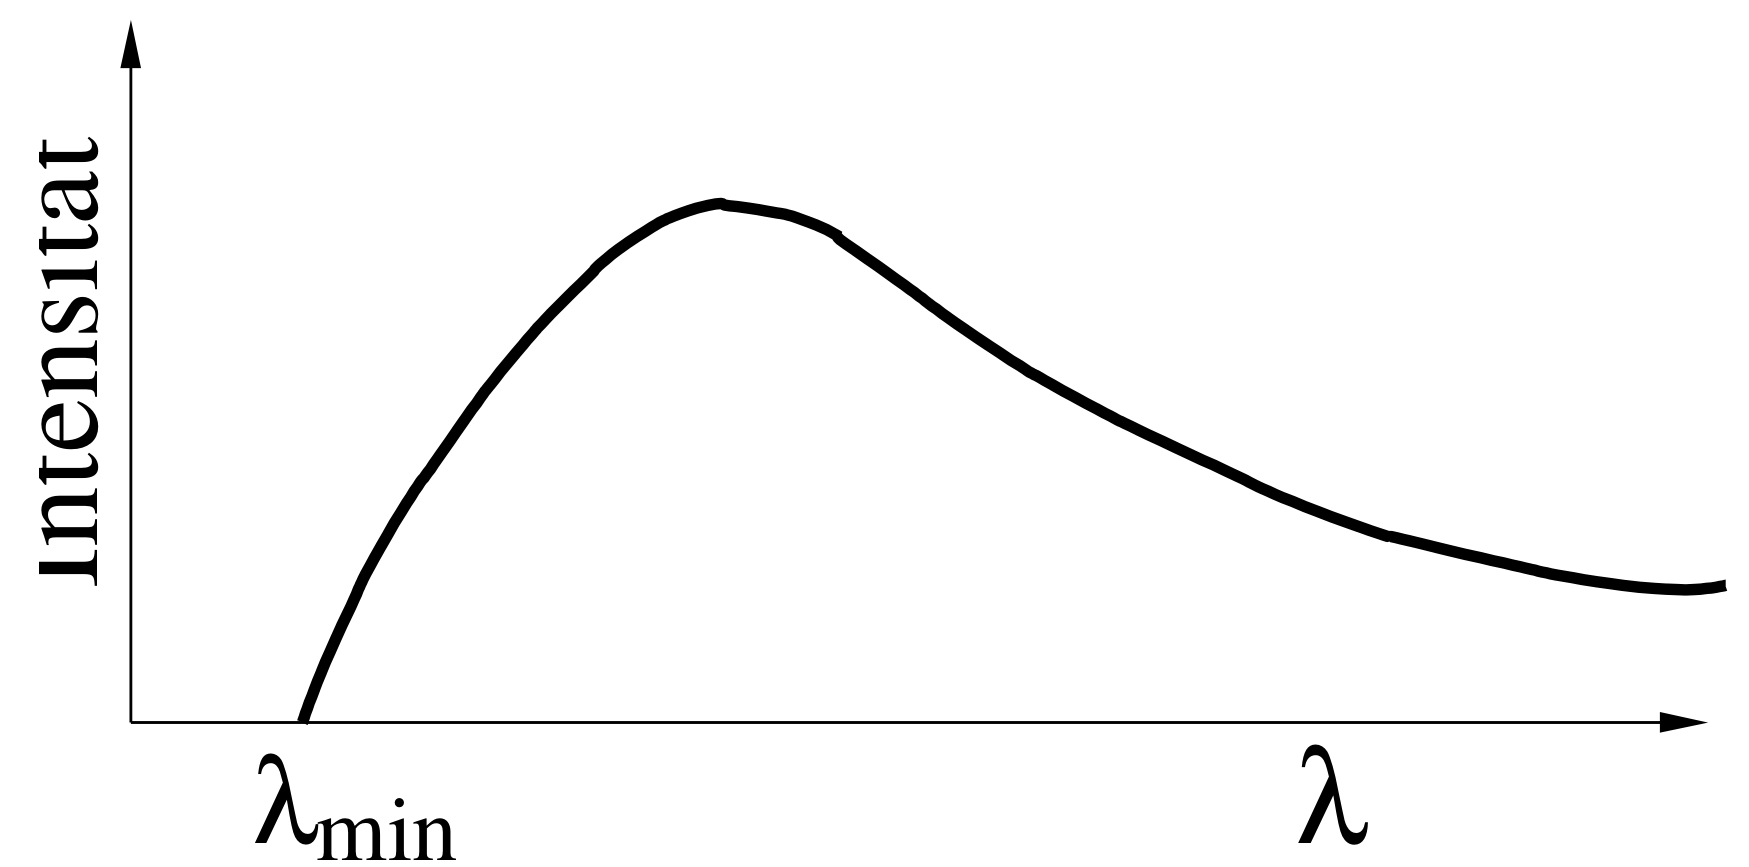
\includegraphics[width=0.5\linewidth]{kontSpektrum.png}
	\caption{Kontinuierliches Bremsspektrum. \cite[1]{anleitung602}}
	\label{fig:kontspekt}
\end{figure}
Die zweite Komponente ist das charakteristische Spektrum, das sich ergibt wenn durch Ionisierung eine freie Stelle in einer inneren Schale eines Atoms entsteht. Um wieder einen energetisch günstigeren Zustand zu erreichen fällt ein Elektron aus einer äußeren Schale
in die Leerstelle. Dabei wird wiederum Energie als ein Röntgenquant abgegeben, wobei die Energie davon abhängig ist, zwischen welchen Schalen gewechselt wurde:

\begin{equation}
h \nu = E_{\text{m}} - E_{\text{n}}.
\end{equation}
Das Spektrum ist also nicht kontinuierlich, da die Energie des Photons nur der Energiedifferenz der jeweiligen Schalen entsprechen kann. Stattdessen setzt es sich aus Linien zusammen, die eine Energie besitzen, welche vom Anodenmaterial abhängt. Die Linien werden 
$K_{\text{$\alpha$}}, K_{\text{$\beta$}}, L_{\text{$\alpha$}}, ...$ genannt. Die Großbuchstaben geben an, auf welche Schale das Elektron wechselt, der Buchstabe im Index steht für die Schale aus der das Elektron kam.

Wird ein Mehrelektronenatom betrachtet, so fällt auf, dass die Elektronen nicht alle dieselbe Bindungsenergie haben. Grund dafür ist, dass Elektronen auf äußeren Schalen von denen auf den inneren abgeschirmt werden und auch unter den Elektronen Wechselwirkungen 
herrschen, sodass äußere Elektronen weniger stark vom Kern angezogen werden als die inneren. Die Bindungsenergie $E_{\text{n}}$ auf der n-ten Schale lässt sich mit der Rydbergenergie $R_{\text{\infty}} = 137{,}6\, \symup{eV}$, der Abschirmkonstanten $\sigma$, 
die für jedes Elektron anders ist, und der effektiven Kernladung $z_{\text{eff}} = z - \sigma$ berechnen:

\begin{equation}
E_{\text{n}} = -R_{\text{\infty}} z_{\text{eff}}^2 \cdot \frac{1}{n^2}.
\end{equation}
Damit ist die Energie $E_{\text{K$\alpha$}}$ der $K\alpha$ -Linie:

\begin{equation}
E_{\text{K$\alpha$}} = R_{\text{\infty}} (z - \sigma_1)^2 \cdot \frac{1}{1^2} - R_{\text{\infty}} (z - \sigma_2)^2 \cdot \frac{1}{2^2}.
\end{equation}

Jede Linie des Spektrums besteht wiederum aus Linien, die nah beisammen liegen. Dies wird als Feinstruktur bezeichnet und kommt durch die Bahndrehimpulse und Spins der Elektronen zustande.


\subsection{Röntgenabsorption}
Auch ist es möglich, dass Röntgenstrahlung absorbiert wird. Wichtige Beispiele sind der Compton- und der Photoeffekt bei Strahlung unter $1\,\symup{MeV}$. Bei der Röntgenabsorption ist zu beobachten, dass bei größer werdenden Energien der Absorptionskoeffizient zunächst
abnimmt. Sobald die Energie des Röntgenquants die Bindungsenergie eines Elektrons der nächsten inneren Schale übersteigt nimmt der Absorptionskoeffizient schlagartig zu. Die Lage der Absorptionskanten $h \nu_{\text{abs}} = E_{\text{n}} - E_{\text{\infty}}$ fallen dabei 
mit der Bindungsenergie zusammen. Je nachdem von welcher Schale das Elektron gewechselt ist, nennt man die Kanten $K-, L-, M-,...$ Absorptionskante.

Wird die Feinstruktur der Kanten einbezogen, so ist es notwendig mit der Sommerfeldschen Feinstrukturformel die Bindungsenergie $E_{\text{n,j}}$ zu berechnen. Hierbei ist $R_{\text{\infty}}$ die Rydbergenergie, $z_{\text{eff}}$ die effektive Kernladungszahl, $\alpha$ 
die Sommerfeldsche Feinstrukturkonstante, $n$ die Hauptquantenzahl und $j$ der Gesamtdrehimpuls des Elektrons:

\begin{equation}
E_{\text{n,j}} = -R_{\text{\infty}} \biggl(z_{\text{eff,1}}^2 \cdot \frac{1}{n^2} + \alpha^2 z_{\text{eff,2}}^4 \cdot \frac{1}{n^3} \biggl(\frac{1}{j+\frac{1}{2}} - \frac{3}{4n} \biggr)\biggr)
\end{equation}

Die Abschirmkonstante $\sigma_{\text{L}}$ der L-Kante kann über die Energiedifferenz $\Delta E_{\text{L}}$ zweier L-Kanten berechnet werden. In diesem Versuch erfolgt diese Berechnung mithilfe der Energiedifferenz $\Delta E_{\text{L}} = E_{\text{L,II}} - E_{\text{L, III}}$,
der Ordnungszahl $Z$, der Rydbergenergie $R_{\text{\infty}}$ und der Feinstruksturkonstanten $\alpha$:

\begin{equation}
\sigma_{\text{L}} = Z- \biggl( \frac{4}{\alpha} \sqrt{\frac{\Delta E_{\text{L}}}{R_{\text{\infty}}}} - \frac{5\Delta E_{\text{L}}}{R_{\text{\infty}}} \biggr)^{\frac{1}{2}}  \biggl(1 + \frac{19}{32} \alpha^2 \frac{\Delta E_{\text{L}}}{R_{\text{\infty}}} \biggr)^{\frac{1}{2}}
\end{equation}

Die Bragg'sche Reflexion kann Auskunft über die Energie $E$ bzw. die Wellenlänge $\lambda$ von Röntgenstrahlung geben. Dazu wird Röntgenstrahlung an einem dreidimensionalen Gitter aus Atomen, hier in einem LiF-Kristall, gebeugt. Unter dem Glanzwinkel $\theta$ 
interferieren die Strahlen konstruktiv miteinander, sodass mit der Gitterkonstanten $d_{\text{LiF}} = 201{,}4\, \symup{pm}$ die gebeugte Wellenlänge $\lambda$ ermittelt werden kann. $n$ ist hierbei die Beugungsordnung:

\begin{equation}
2d sin\theta = n \lambda.
\end{equation}

\begin{figure}[h!]
	\centering
	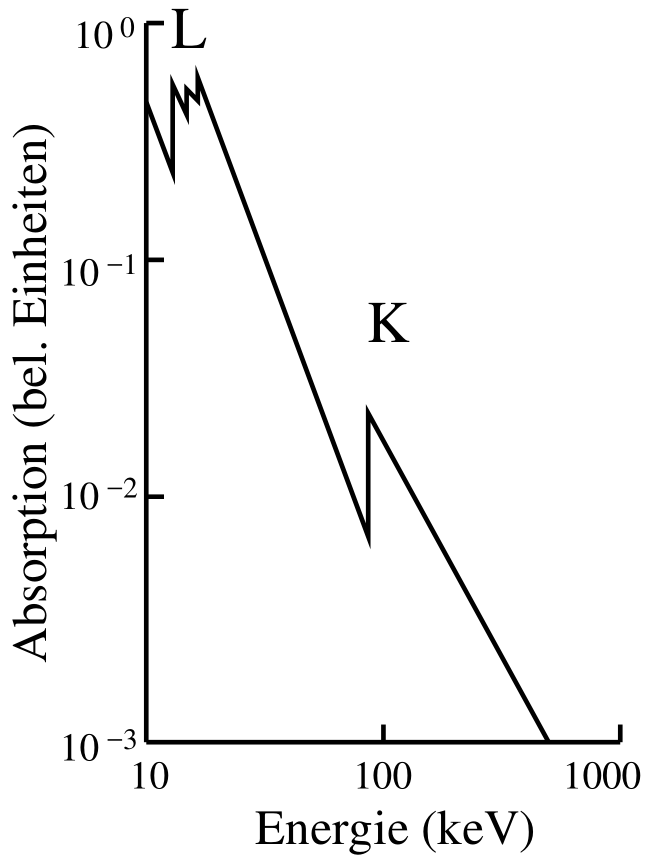
\includegraphics[width=0.4\linewidth]{charSpektrum.png}
	\caption{Absorptionsspektrum. \cite[2]{anleitung602}}
	\label{fig:absorptionsspekt}
\end{figure}